\section{Day 6: Closed Sets, Cantor Construction, Closures and Interiors; Continuity (Sep. 19, 2024)}
Outfit of the day!\footnote{livetexing this sum bitch- so i can't dror pic. sike} Rainbow unicorns owo!
\begin{figure}[h]
    \centering
    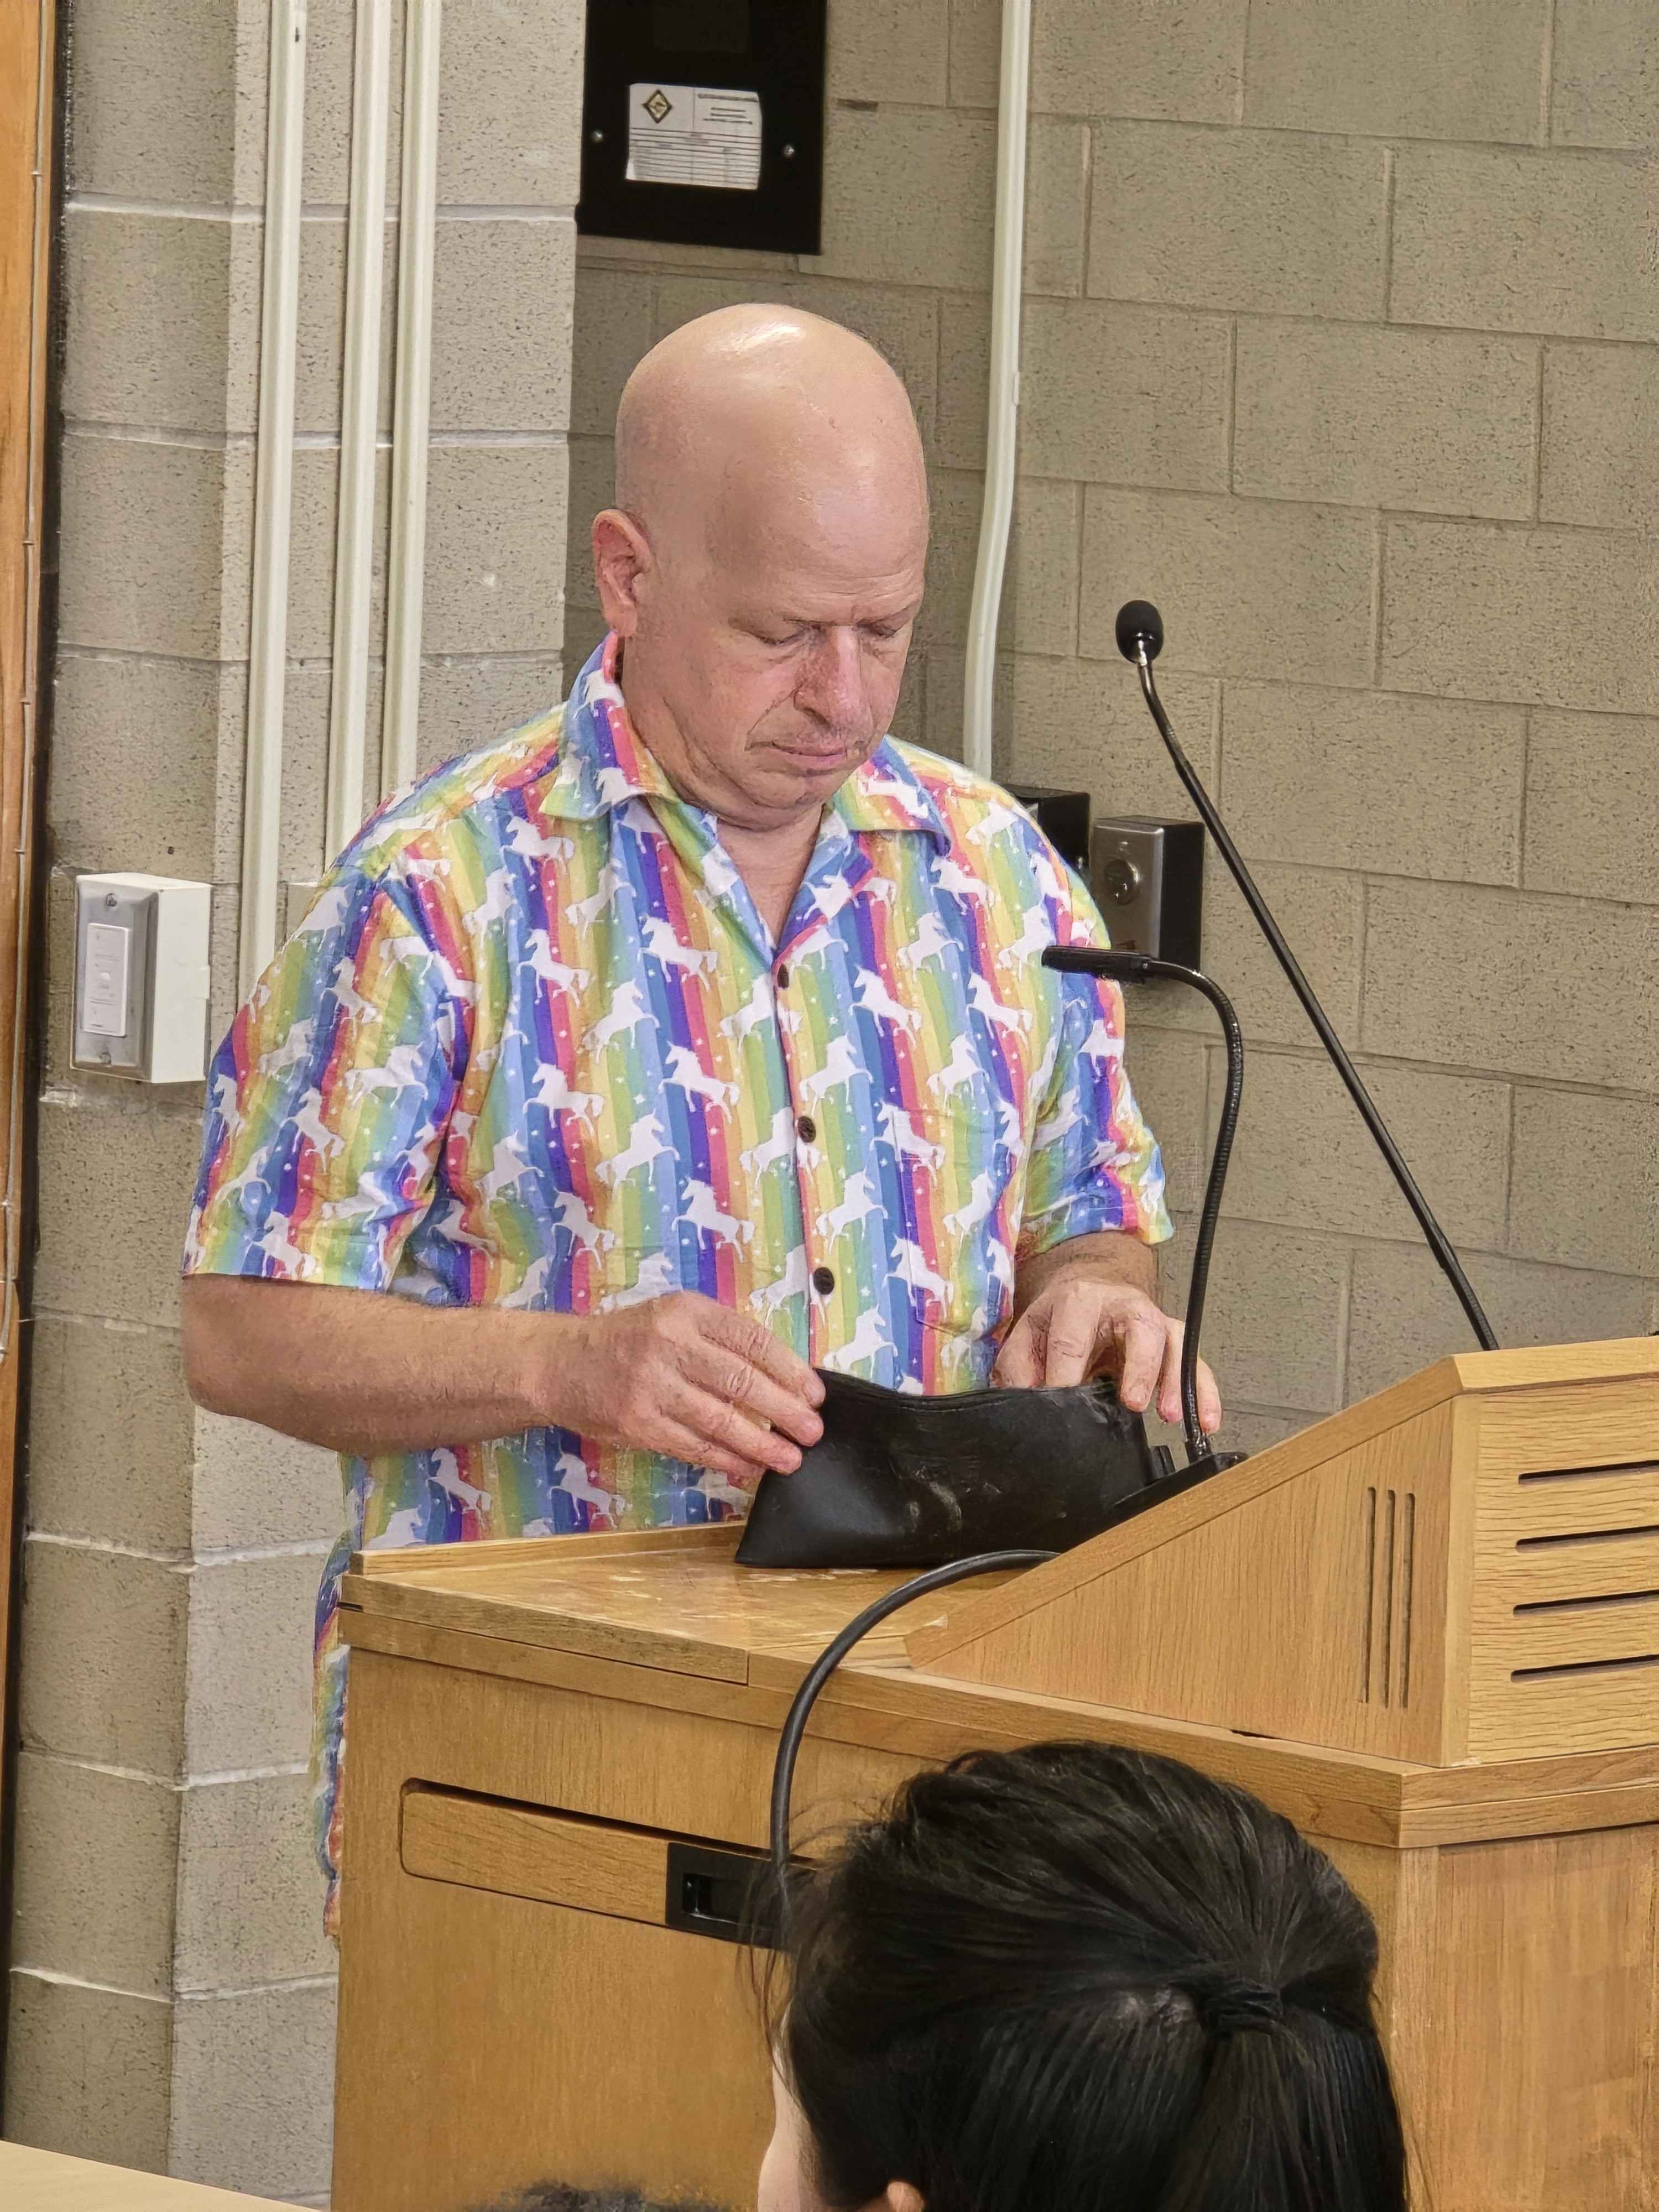
\includegraphics[scale=0.1]{MAT327 Notes/Dror Shirts/dror day 6 shirt.jpg}
\end{figure}

\noindent Course administrative details;
\begin{itemize}
    \item Office hours have been moved to Tuesdays, on 9:30 to 10:30AM.
\end{itemize}

\noindent If $X$ is a topological space, we say that a set $B \subset X$ is closed if its complement, $B^c = X \setminus B$ is open. \textit{Sets are not doors; they can be open, closed, both, or neither.} For example, in the discrete topology, all sets are both open and closed (in general, $\emptyset$ and $X$ are the only sets that are always clopen).
\medskip\newline
Closed sets have the following properties,
\begin{enumerate}[label=(\alph*)]
    \item $\emptyset, X$ are both closed sets.
    \item The arbitary intersection of closed sets is closed.
    \item The finite union of closed sets is closed.
\end{enumerate}
In particular, the last two properties are derived through considering the complements of the union and intersection properties of open sets. Specifically, if $A_\alpha$ is a collection of open sets, then
\[ \left(\bigcup_{\alpha} A_\alpha\right)^c = \bigcap_{\alpha} A_\alpha^c, \hspace{0.2in} \left(\bigcap_{\alpha} A_\alpha \right)^c = \bigcup_\alpha A_\alpha^c. \]
\begin{simplethm}[Continuity, defined by Pre-Images of Closed Sets]
    Any function $F : X \to Y$ (with topological spaces $X, Y$) is continuous if and only if, for every closed $C \subset Y$, we have $f^{-1}(C)$ is closed in $X$.
\end{simplethm}
\noindent To see this, we may write
\[ f^{-1}(C) = f^{-1}((C^c)^c) = f^{-1}(C^c)^c. \]
Since $C^c$ is an open set, we have that $f^{-1}(C^c)$ is open in $X$, and so its complement is closed. This means $f^{-1}(C)$ is closed in $X$. \qed
\begin{remark}
    Having defined continuity, we note that the last two properties of closed sets could have also been used to define the notion of topologies instead of open sets.
\end{remark}
\noindent Now, let us consider the following example: consider $\RR_\mathrm{std}$ containing $C_0 = [0, 1]$. Then $C_0^c = (-\infty, 0) \cup (1, \infty)$. Next, define $C_1 = [0, 1] \setminus (\frac{1}{3}, \frac{2}{3}) = [0, \frac{1}{3}] \cup [\frac{2}{3}, 1]$, i.e. $C_0$ with its inner third removed. Let $C_2$ be $C_1$ with the inner thirds of each of its intervals removed, etc.;
\medskip\newline
\noindent Notice that each $C_n$ is a union of closed intervals on $\RR_\mathrm{std}$. Define
\[ \SC = \bigcap_{n=0}^\infty C_n = [0, 1] \setminus \bigcup_{n=0}^\infty \bigcup_{k=0}^{3n-1} \left(\frac{3k+1}{3^{n+1}}, \frac{3k+2}{3^{n+1}}\right). \]
Since the arbitrary union of open intervals is open, we see that the complement of them is closed, meaning $\SC$ is closed. Moreover, we claim that $\SC$ is not empty. Start by writing $\SC$ as the set $\{x \mid x_3 \text{ has no } 1\text{s}\}$, i.e. $x_3$ representing the ternary expansion of $x$. For any number whose ternary decimal representation consists of only $0$s and $2$s, we may write said number as an infinitely recurring decimal containing $1$, since $0.1\overline{2}_3 = 0.2_3$, by rewriting the last $2$ in the expansion of any such number.
\medskip\newline
\noindent Clearly, $\SC$ is uncountable. In addition, it exhibits the properties,\footnote{read more here ig? \href{https://en.wikipedia.org/wiki/Cantor_set}{linkylinkylink}}
\begin{itemize}
    \item $\SC$ is uncountable, yet the length of $\SC$ is $0$.
    \item \textit{(Originally left as exercise; Devil's Staircase Construction)} There exists a continuous $F : [0, 1] \to [0, 1]$ such that $F(0) = 0, F(1) = 1$ and for all $x \not\in \SC$, we have that $F'(X) = 0$.
    \item \textit{(Originally left as exercise)} What is $\SC + \SC = \{x + y \mid x, y \in \SC\}$? Alternatively, consider $f : \SC \times \SC \to \RR$ where $f(x, y) = x + y$.
\end{itemize}

\newpage
\noindent When is a set closed in the product of two spaces? Suppose $A \subset X, B \subset Y$ are closed sets in their respective topological spaces. Then observe that we cannot just take the complement as follows,
\[ (A \times B)^c \neq A^c \times B^c, \]
since $(A \times B)^c = (A^c \times Y) \cup (X \times B^c)$. Observing that both of these sets are open, we see that $(A \times B)^c$ is also open, meaning $A \times B$ is closed. \qed

\begin{simpleclaim}
    If $Y \subset X$ are topological spaces with $Y$ having the subspace topology, then $C \subset Y$ is closed if and only if there exists some closed $B \subset X$ such that $C = B \cap Y$.
\end{simpleclaim}
\begin{simpleclaim}
    If $Y \subset X$ is closed, and $B \subset Y$ is closed in $Y$, then $B$ is closed in $X$.
\end{simpleclaim}

\noindent We now define the interior and closure of sets.
\begin{itemize}
    \item The interior of $A$ is denoted $\mathrm{int}_X A = \mathring{A}$. It is the largest open set contained in $A$. By the arbitrary union property of open sets, this is given by the union of all open sets contained in $A$.
    \item The closure of $A$, $\mathrm{cl}_X A = \overline{A}$, is the smallest closed set containing $A$, namely the intersection of all closet sets containing $A$.
\end{itemize}
For an example, we have that
\begin{align*}
    [0, 1)^o &= (0, 1), \\
    \overline{[0, 1)} &= [0, 1]. \\
\end{align*}
If $A$ is open, then $\mathring{A} = A$. If $A$ is closed, then $\overline{A} = A$. Here are some more properties on interiors and closures:
\begin{itemize}
    \item The interior of the interior of $A$ is equal to the interior of $A$, i.e. $\mathring{\mathring{A}} = \mathring{A}$.
    \item The same holds for the closure, i.e. $\overline{\overline{A}} = \overline{A}$.
    \item The interior and closure of any clopen set is the clopen set itself. For example, $\mathring{\emptyset} = \overline{\emptyset} = \emptyset$, and the same holds for the whole set.
    \item In general, we don't know what $\mathring{\overline{A}}$ or $\overline{\mathring{A}}$ is.
    \item The complement of $\overline{A}$ is given by
    \[ \overline{A}^c = \left(\bigcap_{\substack{F \supset A \\ F \text{ closed}}} F \right)^c = \bigcup_{\substack{F \supset A \\ F \text{ closed}}} F = \bigcup_{\substack{U^c \supset A \\ U^c \text{ closed}}} U \underbrace{=}_{F^c = U} \bigcup_{\substack{U \subset A^c \\ U \text{ open}}} U = \mathring{(A^c)}. \]
    Thus, the complement of the closure is the interior of the complement.
    \item Likewise, we have $(\mathring{A})^c = \overline{A^c}$.
    \item \textit{(Challenge Exercise)} Prove that we can make $14$ distinct sets from any general set $A$ using complement, closure, and interior.
\end{itemize}

\newpage
\begin{simplethm}
    Let $X$ be a topological space, and let $A \subset X$. $x$ is in the closure of $A$ if and only if every neighborhood of $x$ intersects $A$. A neighborhood of $x$ is defined as an open set containing $x$.
\end{simplethm}
\noindent Specifically, the condition above may be written as $\forall U \in \ST_X$, we have $x \in U \implies U \cap A \neq \emptyset$.
\begin{itemize}
    \item[$(\Rightarrow)$] Assume $x \in \overline{A}$ by contradiction. Assume that $U$ is open and $x \in U$, with $U \cap A = \emptyset$. We have $U^c \supset A$, but $U^C$ is closed. Since $x \not\in U^c \supset \overline{A} \ni x$ is a contradiction, we are done.
    \item[$(\Leftarrow)$] Assume every neighborhood of $X$ intersects $A$. By contradiction, also assume that $x \not\in \overline{A}$. Then $\overline{A}^c \ni x$ is a neighborhood of $x$, not intersecting $A$. This is a contradiction, so we are done. \qed
\end{itemize}
In fact, we may check basic neighborhoods (i.e., open set in basis containing $x$) only instead of all neighborhoods.

\begin{simpleclaim}[Closure of $\QQ$ is $\RR$]
    We have that $\overline{Q} = \RR$.
\end{simpleclaim}
\noindent For all $x \in \RR$, we have $x \in \overline{\QQ}$ if and only if $x \in (a, b)$ implies $(a, b) \cap \QQ \neq \QQ$. \qed

\begin{definition}
    Given $A \subset X$, $x \in X$ is a limit of $A$ if every neighborhood of $x$ contains a point of $A$ other than $x$ itself. This is equivalent to saying that $x \in \overline{A \setminus \{x\}}$.
\end{definition}

\begin{simplethm}
    $\overline{A} = A \cup A'$ where $A'$ is given by the set of limit points of $A$.
\end{simplethm}
\begin{itemize}
    \item[$(\supset)$] $\overline{A} \supset A$ is trivially true. If $x \in A'$, then $x \in \overline{A \setminus \{x\}} \subset \overline{A}$.
    \item[$(\subset)$] Take $x \in \overline{A}$. If $x \in A$, we're automatically done. Thus, let us assume that $x \not\in A$; then $x \in \overline{A} = \overline{A \setminus \{x\}}$, implying that $x \in A'$. \qed
\end{itemize}
We now present a fheorem (false theorem). If $x$ is a limit point of some set $A$, then every neighborhood of $x$ contains infinitely many elements of $A$, i.e.
\[ x \in U \in \ST_X \implies \abs{U \cap A} = \infty. \]
We now present a froof (false proof). For any $x$, we may take any neighborhood about $x$. Then we may remove a point $a_1$; since the neighborhood with $a_1$ removed is still an open set, we may remove $a_2$, $a_3$, and so on inductively. \qed